%%%%%%%%%%%%%%%%%%%%%%%%%%%%%%%%%%%%%%%%%%%%%%%%%%%%%%%%%%
% # Appendix: Elicited Production Task Results
%%%%%%%%%%%%%%%%%%%%%%%%%%%%%%%%%%%%%%%%%%%%%%%%%%%%%%%%%%

\chapter{Elicited Production Task Results}\label{app-results-ept}

%========================================================%
\section{Response rates}\label{app-ept-token}
%========================================================%

% ORC Means
% \DTLloaddb{dt-ept-token}{../analysis/tables/ept_token.csv}
% \ExplSyntaxOn
% \tl_new:N \tblrbody
% \tl_build_begin:N \tblrbody
% \DTLforeach[\equal{\col}{ORC}]{dt-ept-token}{\col=study,\coli=Group,\colii=Environment,\coliii=Dependency,\coliv=Mean,\colv=$CI$,\colvi=Percent}{\tl_build_put_right:Ne \tblrbody {\exp_not:V \coli & \exp_not:V \colii & \exp_not:V \coliii & \exp_not:V \coliv & \exp_not:V \colv & \exp_not:V \colvi\\}}
% \tl_build_end:N \tblrbody
% \ExplSyntaxOff
% \begin{longtblr}[caption={Mean tokens by participant in the ORC elicited production task}, label={tblr:app-orc-ept-token}, expand=\tblrbody]{colspec={XXXX[r]X[r]X[r]}}\toprule
% Group & Environment & Dependency & Mean & 95\% \textit{CI} & \%\\\midrule
% \tblrbody\bottomrule
% \end{longtblr}
% \vspace{-12pt}

% SRC Means
% \ExplSyntaxOn
% \tl_clear:N \tblrbody
% \tl_build_begin:N \tblrbody
% \DTLforeach[\equal{\col}{SRC}]{dt-ept-token}{\col=study,\coli=Group,\colii=Environment,\coliii=Dependency,\coliv=Mean,\colv=$CI$,\colvi=Percent}{\tl_build_put_right:Ne \tblrbody {\exp_not:V \coli & \exp_not:V \colii & \exp_not:V \coliii & \exp_not:V \coliv & \exp_not:V \colv & \exp_not:V \colvi\\}}
% \tl_build_end:N \tblrbody
% \ExplSyntaxOff
% \begin{longtblr}[caption={Mean tokens by participant in the SRC elicited production task}, label={tblr:app-src-ept-token}, expand=\tblrbody]{colspec={XXXX[r]X[r]X[r]}}\toprule
% Group & Environment & Dependency & Mean & 95\% \textit{CI} & \%\\\midrule
% \tblrbody\bottomrule
% \end{longtblr}
% \vspace{-12pt}

% ORC Figure
% \begin{figure}
% \caption{Mean tokens by participant in the ORC elicited production task} \label{fig:app-orc-ept-token}
% \raggedright\setstretch{1}
% 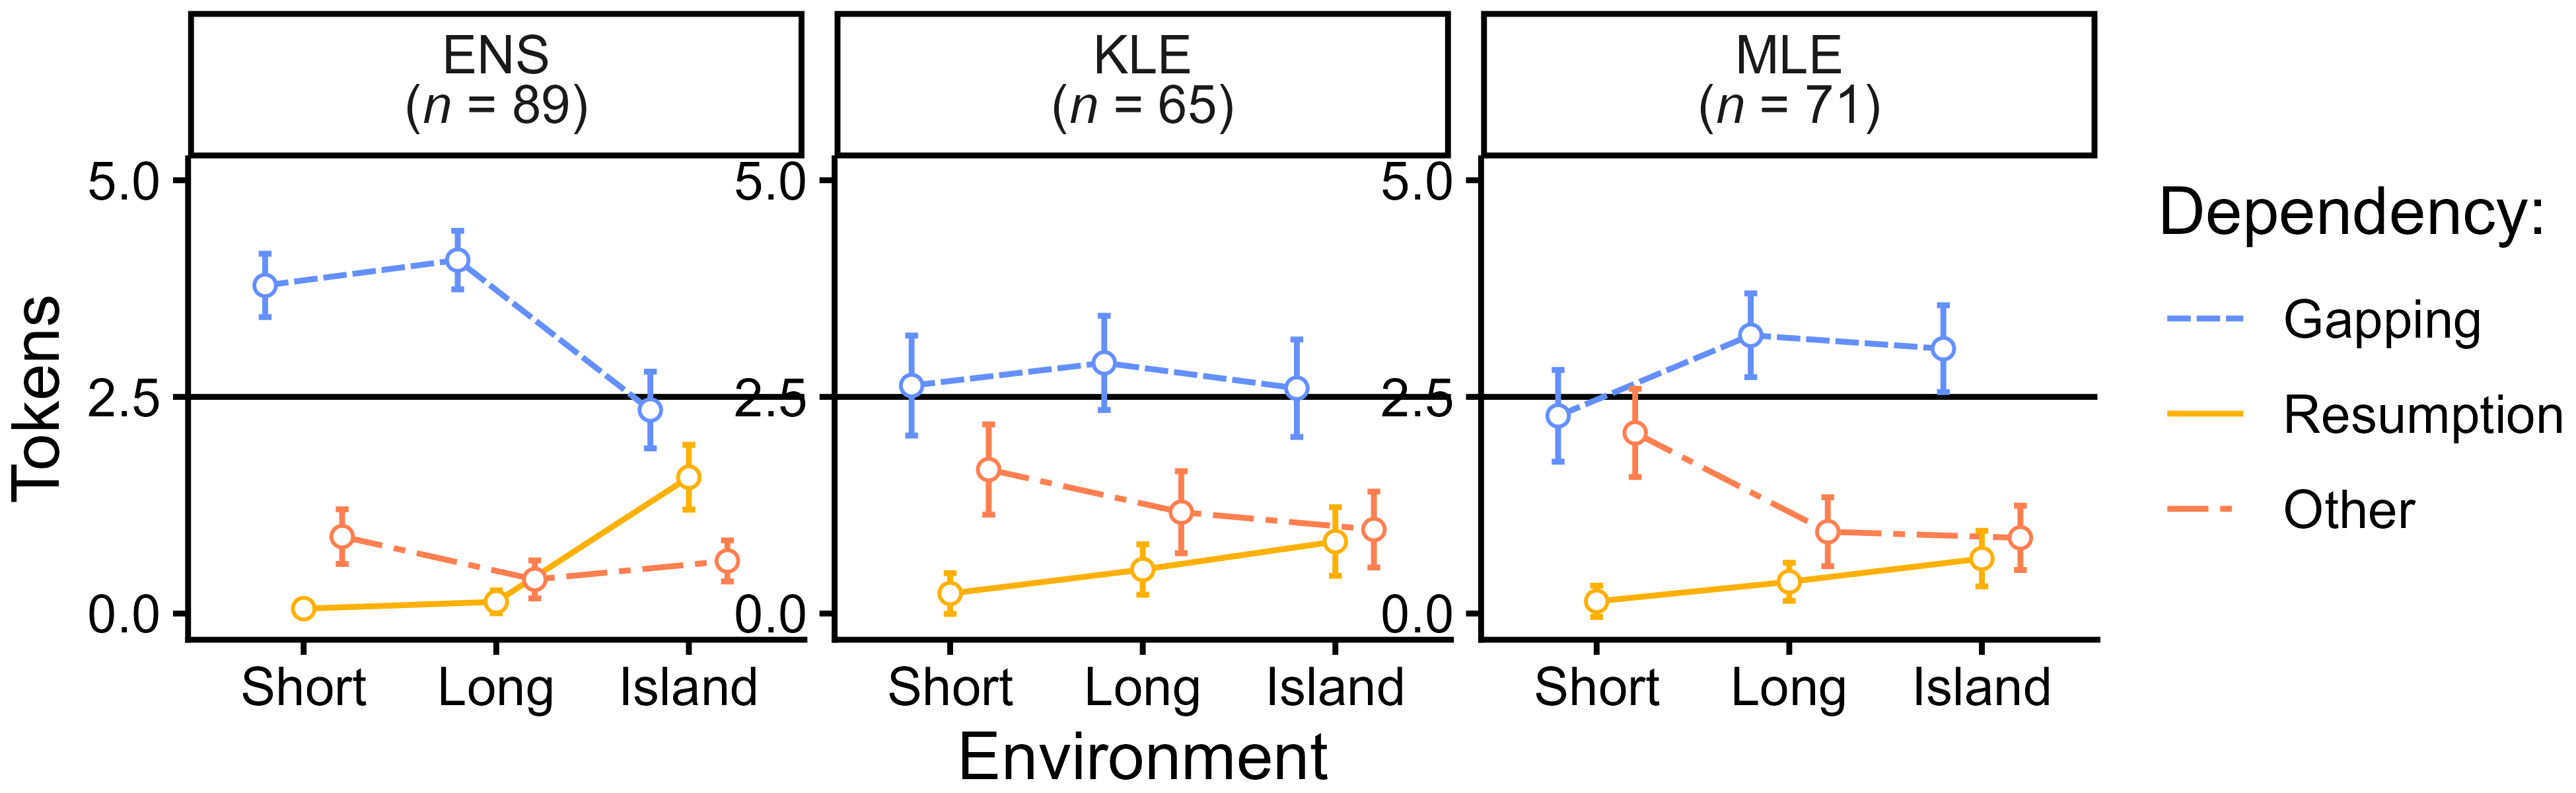
\includegraphics{../analysis/plots/orc_ept_token.png}
% \textit{Note}. Error bars are 95\% $CI$s; center line corresponds to a 50\% response rate.
% \vspace{-12pt}
% \end{figure}

% SRC Figure
% \begin{figure}
% \caption{Mean tokens by participant in the SRC elicited production task} \label{fig:app-src-ept-token}
% \raggedright\setstretch{1}
% 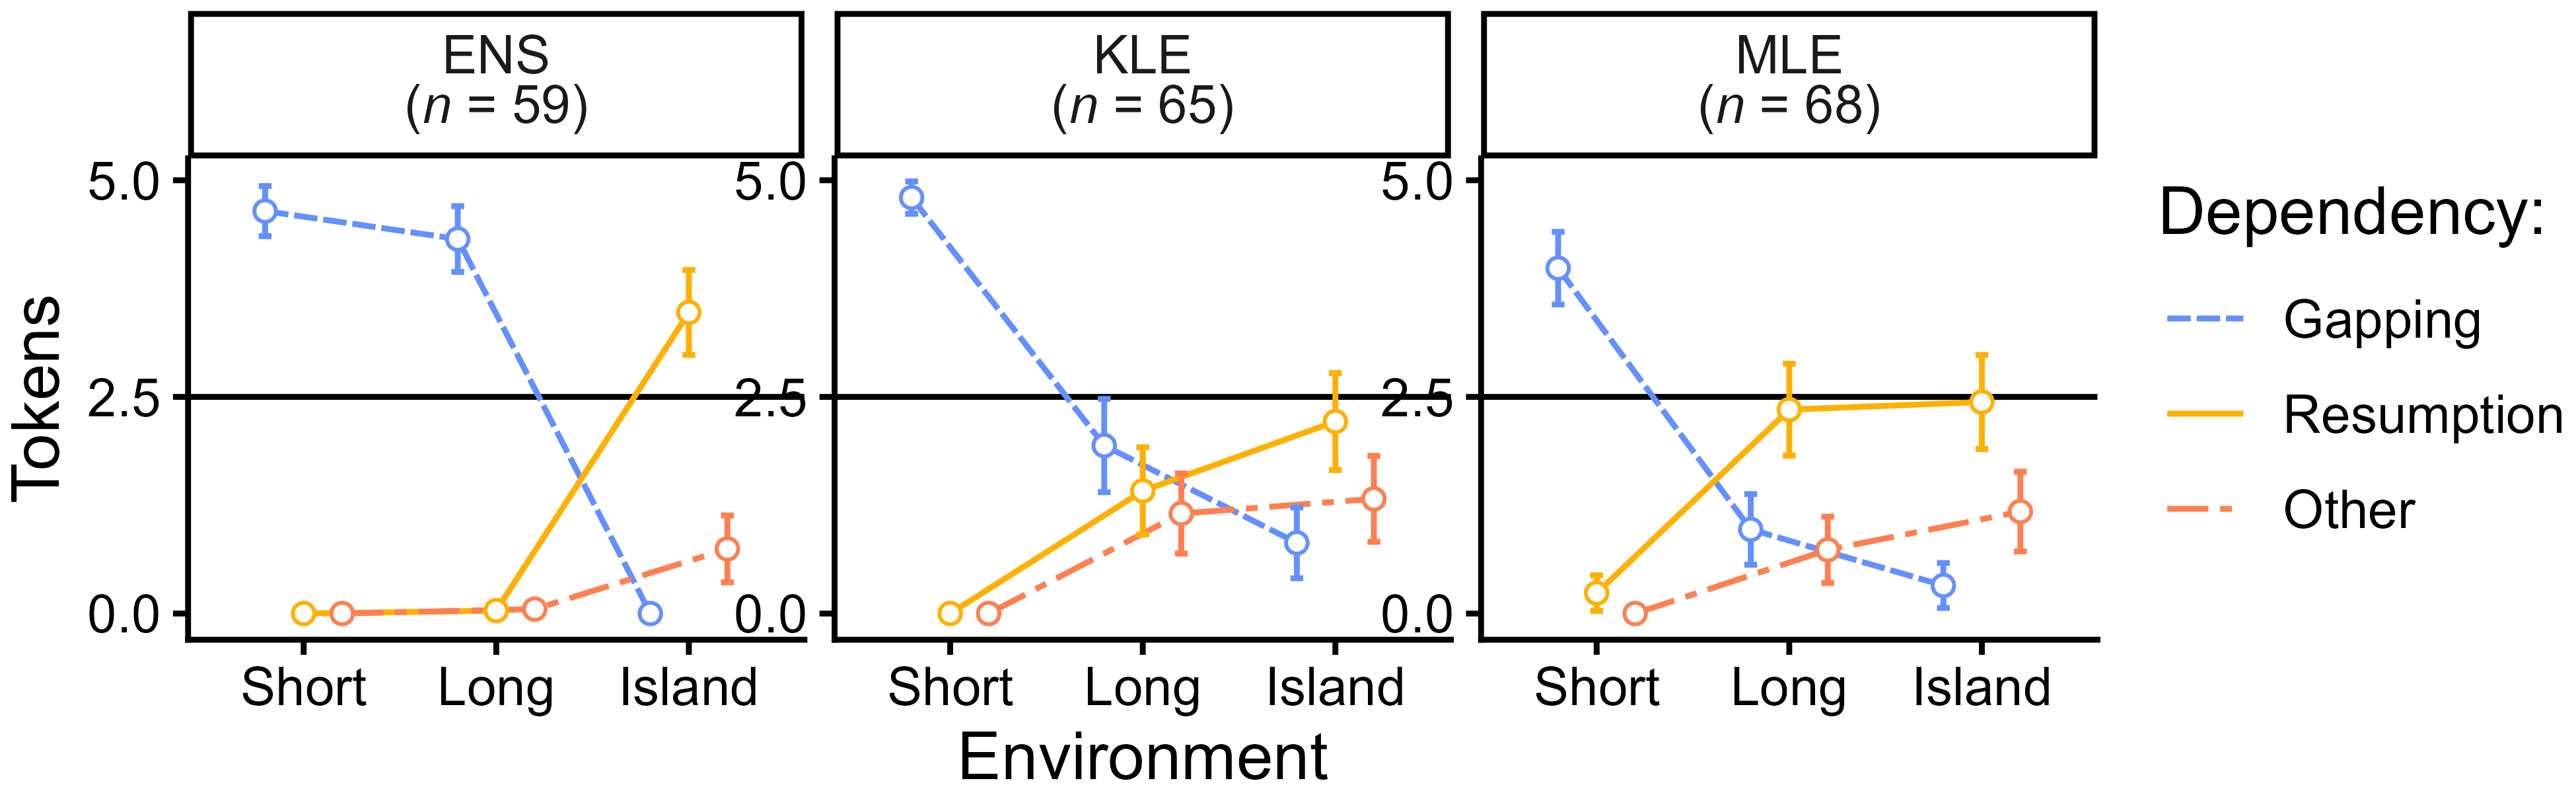
\includegraphics{../analysis/plots/src_ept_token.png}
% \textit{Note}. Error bars are 95\% $CI$s; center line corresponds to a 50\% response rate.
% \vspace{-12pt}
% \end{figure}

% ORC Model
\begin{table}
\caption{Summary of mixed-effects logistic regression model on resumption rates in the ORC elicited production task}\label{tab:app-orc-ept-resumption-model}
\raggedright\setstretch{1}
\begin{tabularx}{\textwidth}{lYYYY}\toprule
Parameter & Estimate~($\hat{\beta}$) & \textit{SE} & $z$ & $p$ \\\midrule
\csvreader[late after line=\\,late after last line=\\\bottomrule]
{../analysis/tables/orc_ept_resumption_model.csv}{}{\csvcoli & \csvcolii & \csvcoliii & \csvcoliv & \csvcolv}
\end{tabularx}
\textit{Note}. Model formula: Resumption \~{} Environment * Group + (1 | Participant) + (1 + Environment + Group | Item); reference level: Short + ENS; estimate unit: logit; intercept: grand mean.
\vspace{-12pt}
\end{table}

% ORC Posthoc
\begin{table}
\caption{Post-hoc tests for resumption rates in the ORC elicited production task}\label{tab:app-orc_ept_resumption_posthoc}
\raggedright\setstretch{1}
\begin{tabularx}{\textwidth}{llYYYY}\toprule
Group~~ & Contrast & Estimate $\hat{\beta}$ & \textit{SE} & $z$ & $p$ \\\midrule
\csvreader[late after line=\\,late after last line=\\\bottomrule]
{../analysis/tables/orc_ept_resumption_posthoc.csv}{}{\csvcoli & \csvcolii & \csvcoliii & \csvcoliv & \csvcolv & \csvcolvi}
\end{tabularx}
\textit{Note}. Adjustment to $p$-values done via multiple $t$ method for 9 tests.
\vspace{-12pt}
\end{table}

% SRC Model
\begin{table}
\caption{Summary of mixed-effects logistic regression model on resumption rates in the SRC elicited production task}\label{tab:app-src-ept-resumption-model}
\raggedright\setstretch{1}
\begin{tabularx}{\textwidth}{lYYYY}\toprule
Parameter & Estimate~($\hat{\beta}$) & \textit{SE} & $z$ & $p$ \\\midrule
\csvreader[late after line=\\,late after last line=\\\bottomrule]
{../analysis/tables/src_ept_resumption_model.csv}{}{\csvcoli & \csvcolii & \csvcoliii & \csvcoliv & \csvcolv}
\end{tabularx}
\textit{Note}. Model formula: Resumption \~{} Environment * Group + (1 + Environment | Participant) + (1 | Item); reference level: Long + ENS; estimate unit: logit; intercept: grand mean.
\vspace{-12pt}
\end{table}

% SRC Posthoc
\begin{table}
\caption{Post-hoc tests for resumption rates in the SRC elicited production task}\label{tab:app-src_ept_resumption_posthoc}
\raggedright\setstretch{1}
\begin{tabularx}{\textwidth}{llYYYY}\toprule
Group~~ & Contrast & Estimate $\hat{\beta}$ & \textit{SE} & $z$ & $p$ \\\midrule
\csvreader[late after line=\\,late after last line=\\\bottomrule]
{../analysis/tables/src_ept_resumption_posthoc.csv}{}{\csvcoli & \csvcolii & \csvcoliii & \csvcoliv & \csvcolv & \csvcolvi}
\end{tabularx}
\textit{Note}. Adjustment to $p$-values done via multiple $t$ method for 3 tests.
\vspace{-12pt}
\end{table}

%========================================================%
% \section{Resumption subtypes}\label{app-ept-subtype}
%========================================================%

% ORC Proportions
% \begin{table}
% \caption{Production rates for resumption subtypes in the ORC elicited production task}\label{tab:app-orc-ept-subtype}
% \raggedright\setstretch{1}
% \begin{tabularx}{\textwidth}{XXYY}\toprule
% Group & Type & Count & \% \\\midrule
% \csvreader[late after line=\\,late after last line=\\\bottomrule]
% {../analysis/tables/orc_ept_subtype.csv}{}{\csvcolii & \csvcoliii & \csvcoliv & \csvcolv}
% \end{tabularx}
% \vspace{-12pt}
% \end{table}

% SRC Proportions
% \begin{table}
% \caption{Production rates for resumption subtypes in the SRC elicited production task}\label{tab:app-src-ept-subtype}
% \raggedright\setstretch{1}
% \begin{tabularx}{\textwidth}{XXYY}\toprule
% Group & Type & Count & \% \\\midrule
% \csvreader[late after line=\\,late after last line=\\\bottomrule]
% {../analysis/tables/src_ept_subtype.csv}{}{\csvcolii & \csvcoliii & \csvcoliv & \csvcolv}
% \end{tabularx}
% \end{table}

%========================================================%
\section{Identification of potentially quotative responses}\label{app-ept-quotative}
%========================================================%

\begin{figure}
\caption{Means of the by-participant response rates in the ORC elicited production task after removing participants with many potentially quotative responses} \label{fig:app-ept-token-orc-quotative}
\raggedright\setstretch{1}
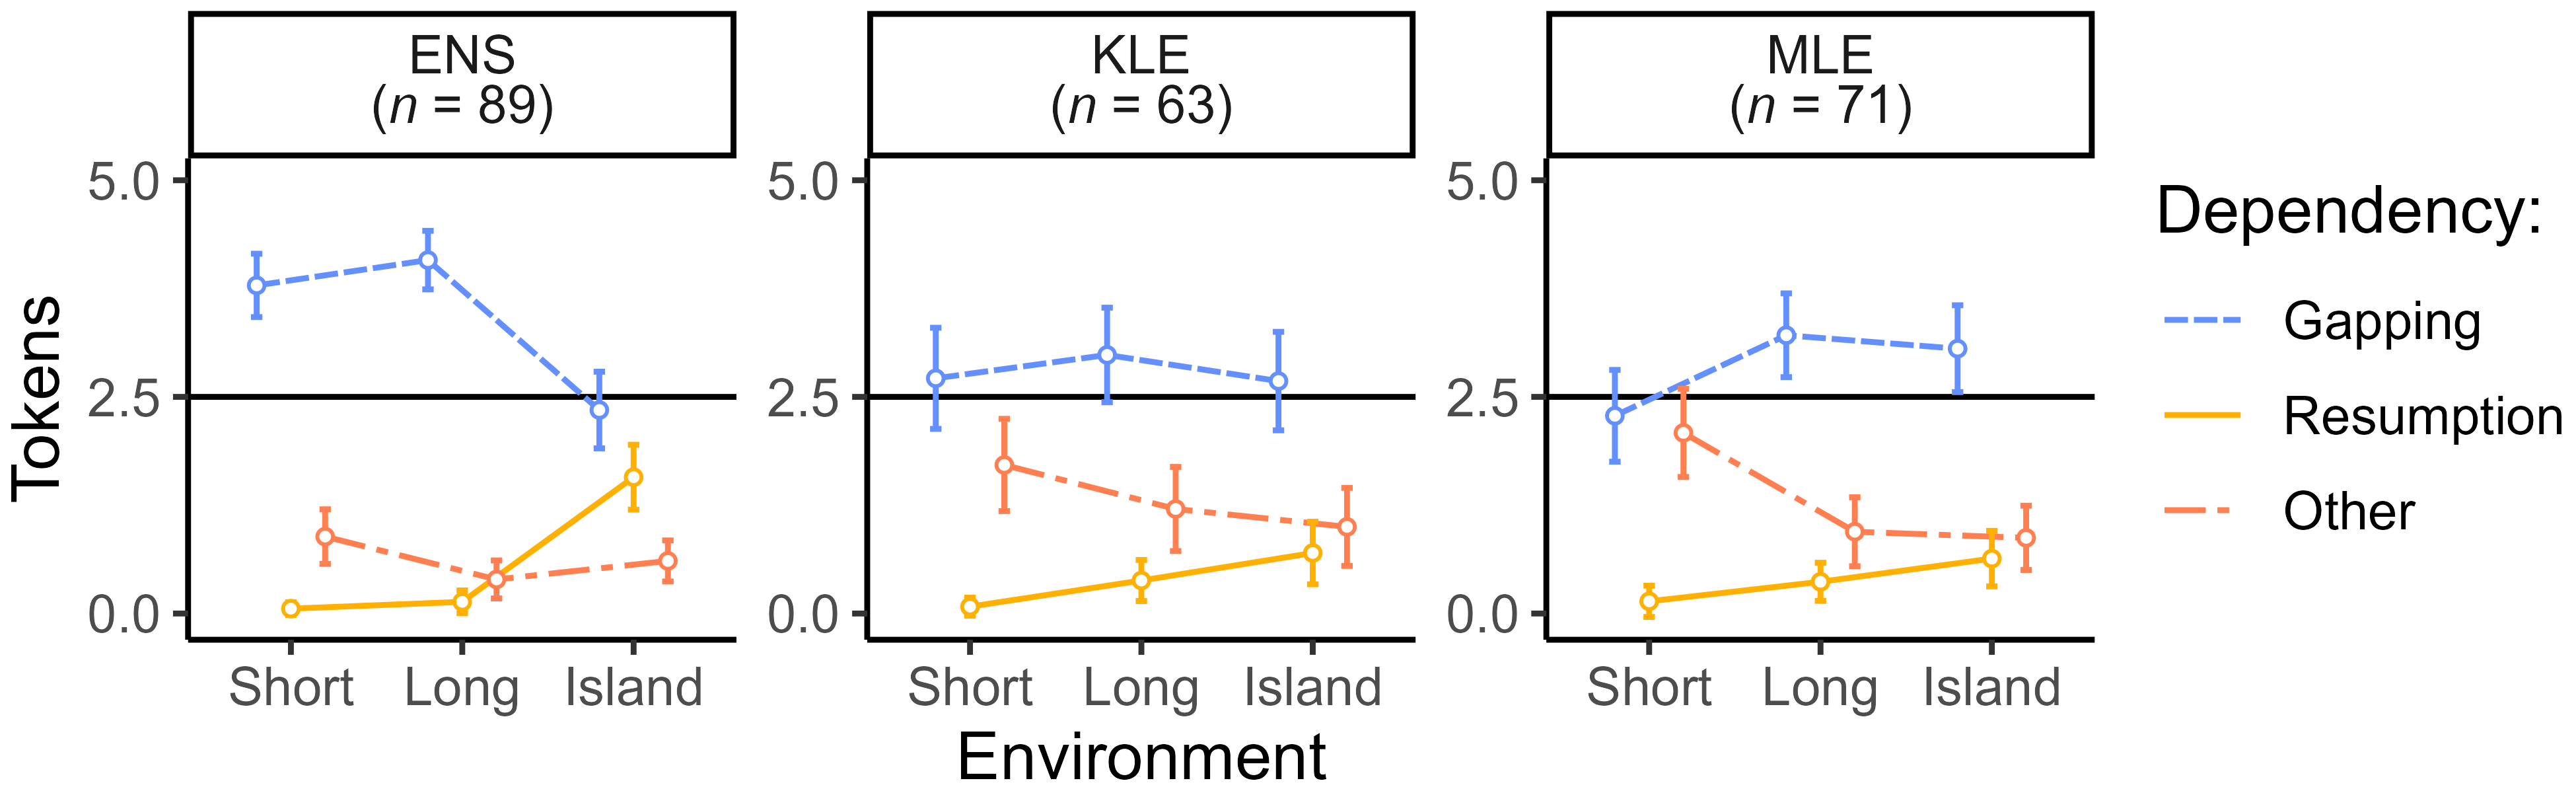
\includegraphics{../analysis/plots/orc_ept_token_quotative.png}
\textit{Note}. Max = 5 tokens per condition; error bars are 95\% \textit{CI}s; center line represents 50\% of responses; Nontarget responses are omitted.
\vspace{-12pt}
\end{figure}

\begin{figure}
\caption{Means of the by-participant response rates in the SRC elicited production task after removing participants with many potentially quotative responses} \label{fig:app-ept-token-src-quotative}
\raggedright\setstretch{1}
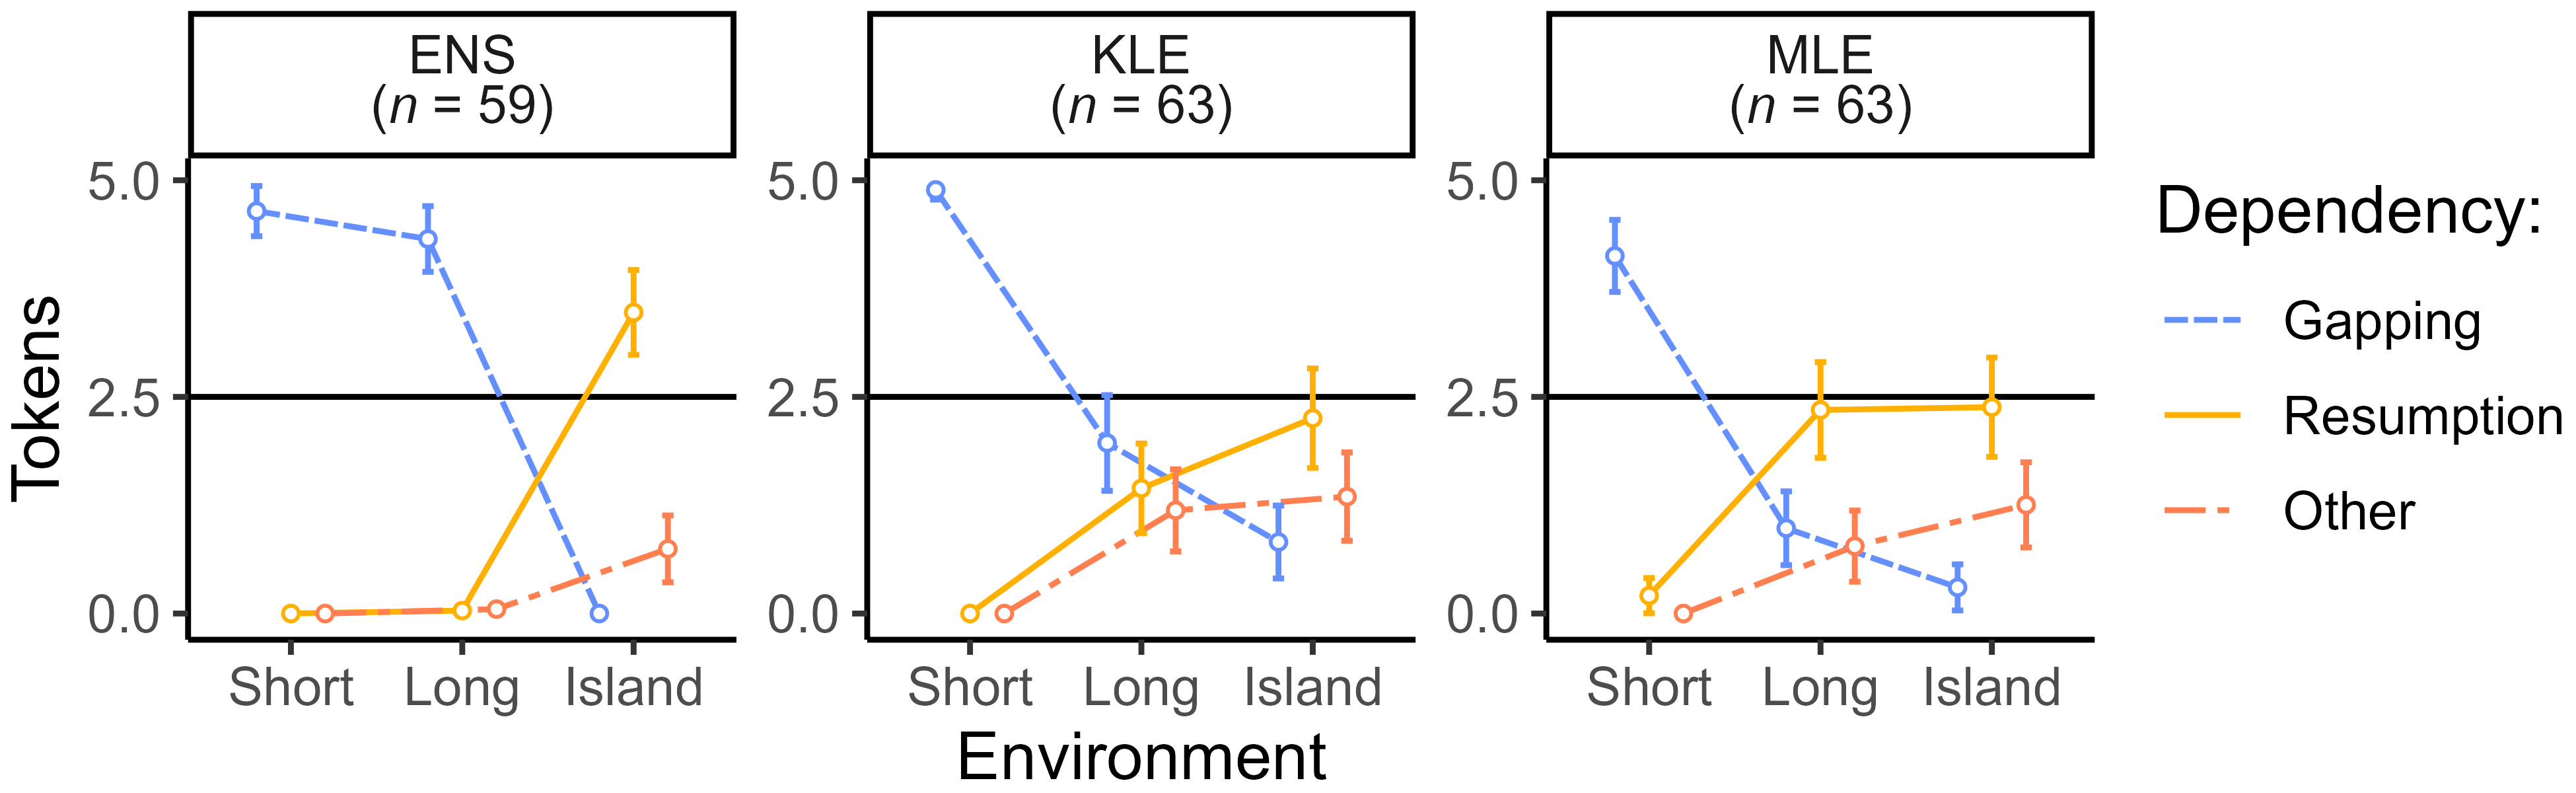
\includegraphics{../analysis/plots/src_ept_token_quotative.png}
\textit{Note}. Max = 5 tokens per condition; error bars are 95\% \textit{CI}s; center line represents 50\% of responses; Nontarget responses are omitted.
\vspace{-12pt}
\end{figure}

\begin{figure}
\caption{Means of the by-participant response rates in the ORC elicited production task after recoding Full~NP responses as Nontarget} \label{fig:app-ept-token-orc-quotative2}
\raggedright\setstretch{1}
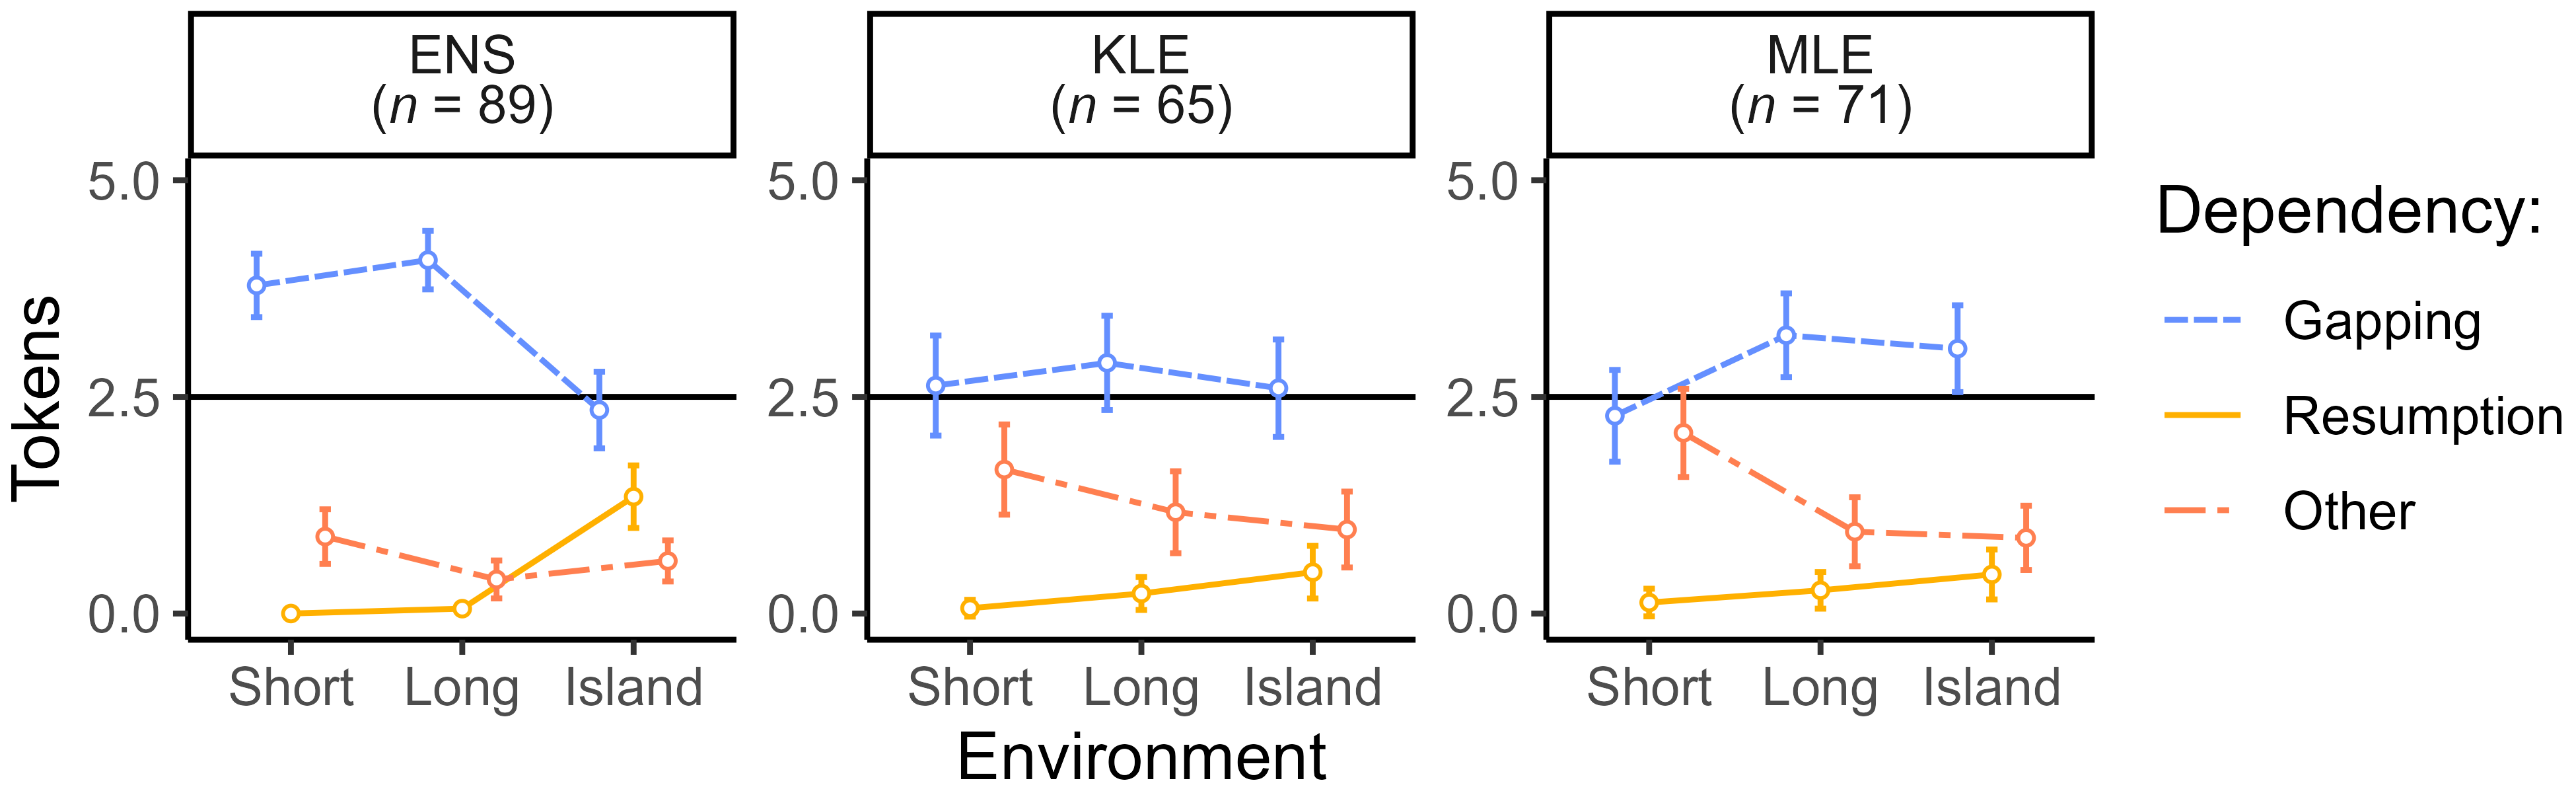
\includegraphics{../analysis/plots/orc_ept_token_quotative2.png}
\textit{Note}. Max = 5 tokens per condition; error bars are 95\% \textit{CI}s; center line represents 50\% of responses; Nontarget responses are omitted.
\vspace{-12pt}
\end{figure}

\begin{figure}
\caption{Means of the by-participant response rates in the SRC elicited production task after recoding Full~NP responses as Nontarget} \label{fig:app-ept-token-src-quotative2}
\raggedright\setstretch{1}
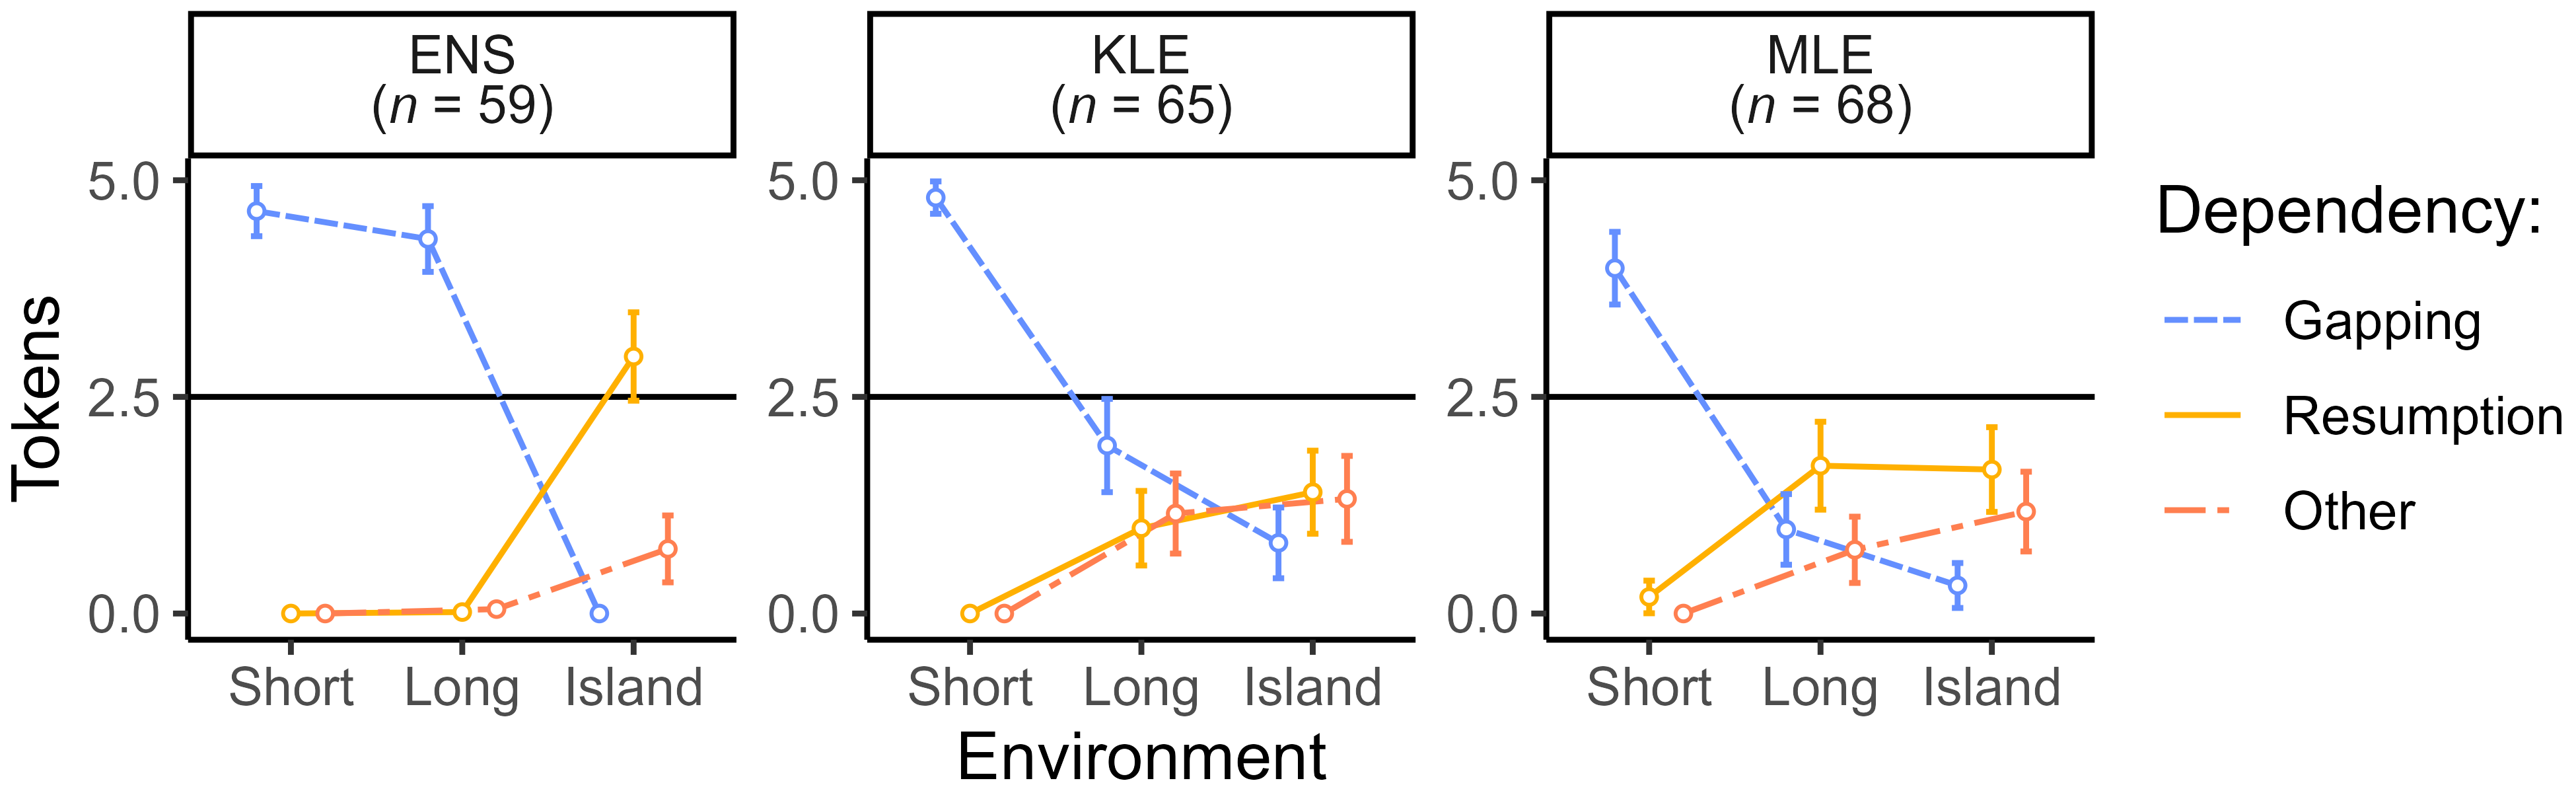
\includegraphics{../analysis/plots/src_ept_token_quotative2.png}
\textit{Note}. Max = 5 tokens per condition; error bars are 95\% \textit{CI}s; center line represents 50\% of responses; Nontarget responses are omitted.
\vspace{-12pt}
\end{figure}

%========================================================%
\section{L2 proficiency effects for resumption rates}\label{app-ept-token-proficiency}
%========================================================%

% ORC Figure
% \begin{figure}
% \caption{Relationship between L2 proficiency and response rates in the ORC elicited production task} \label{fig:app-orc-ept-token-proficiency}
% \raggedright\setstretch{1}
% 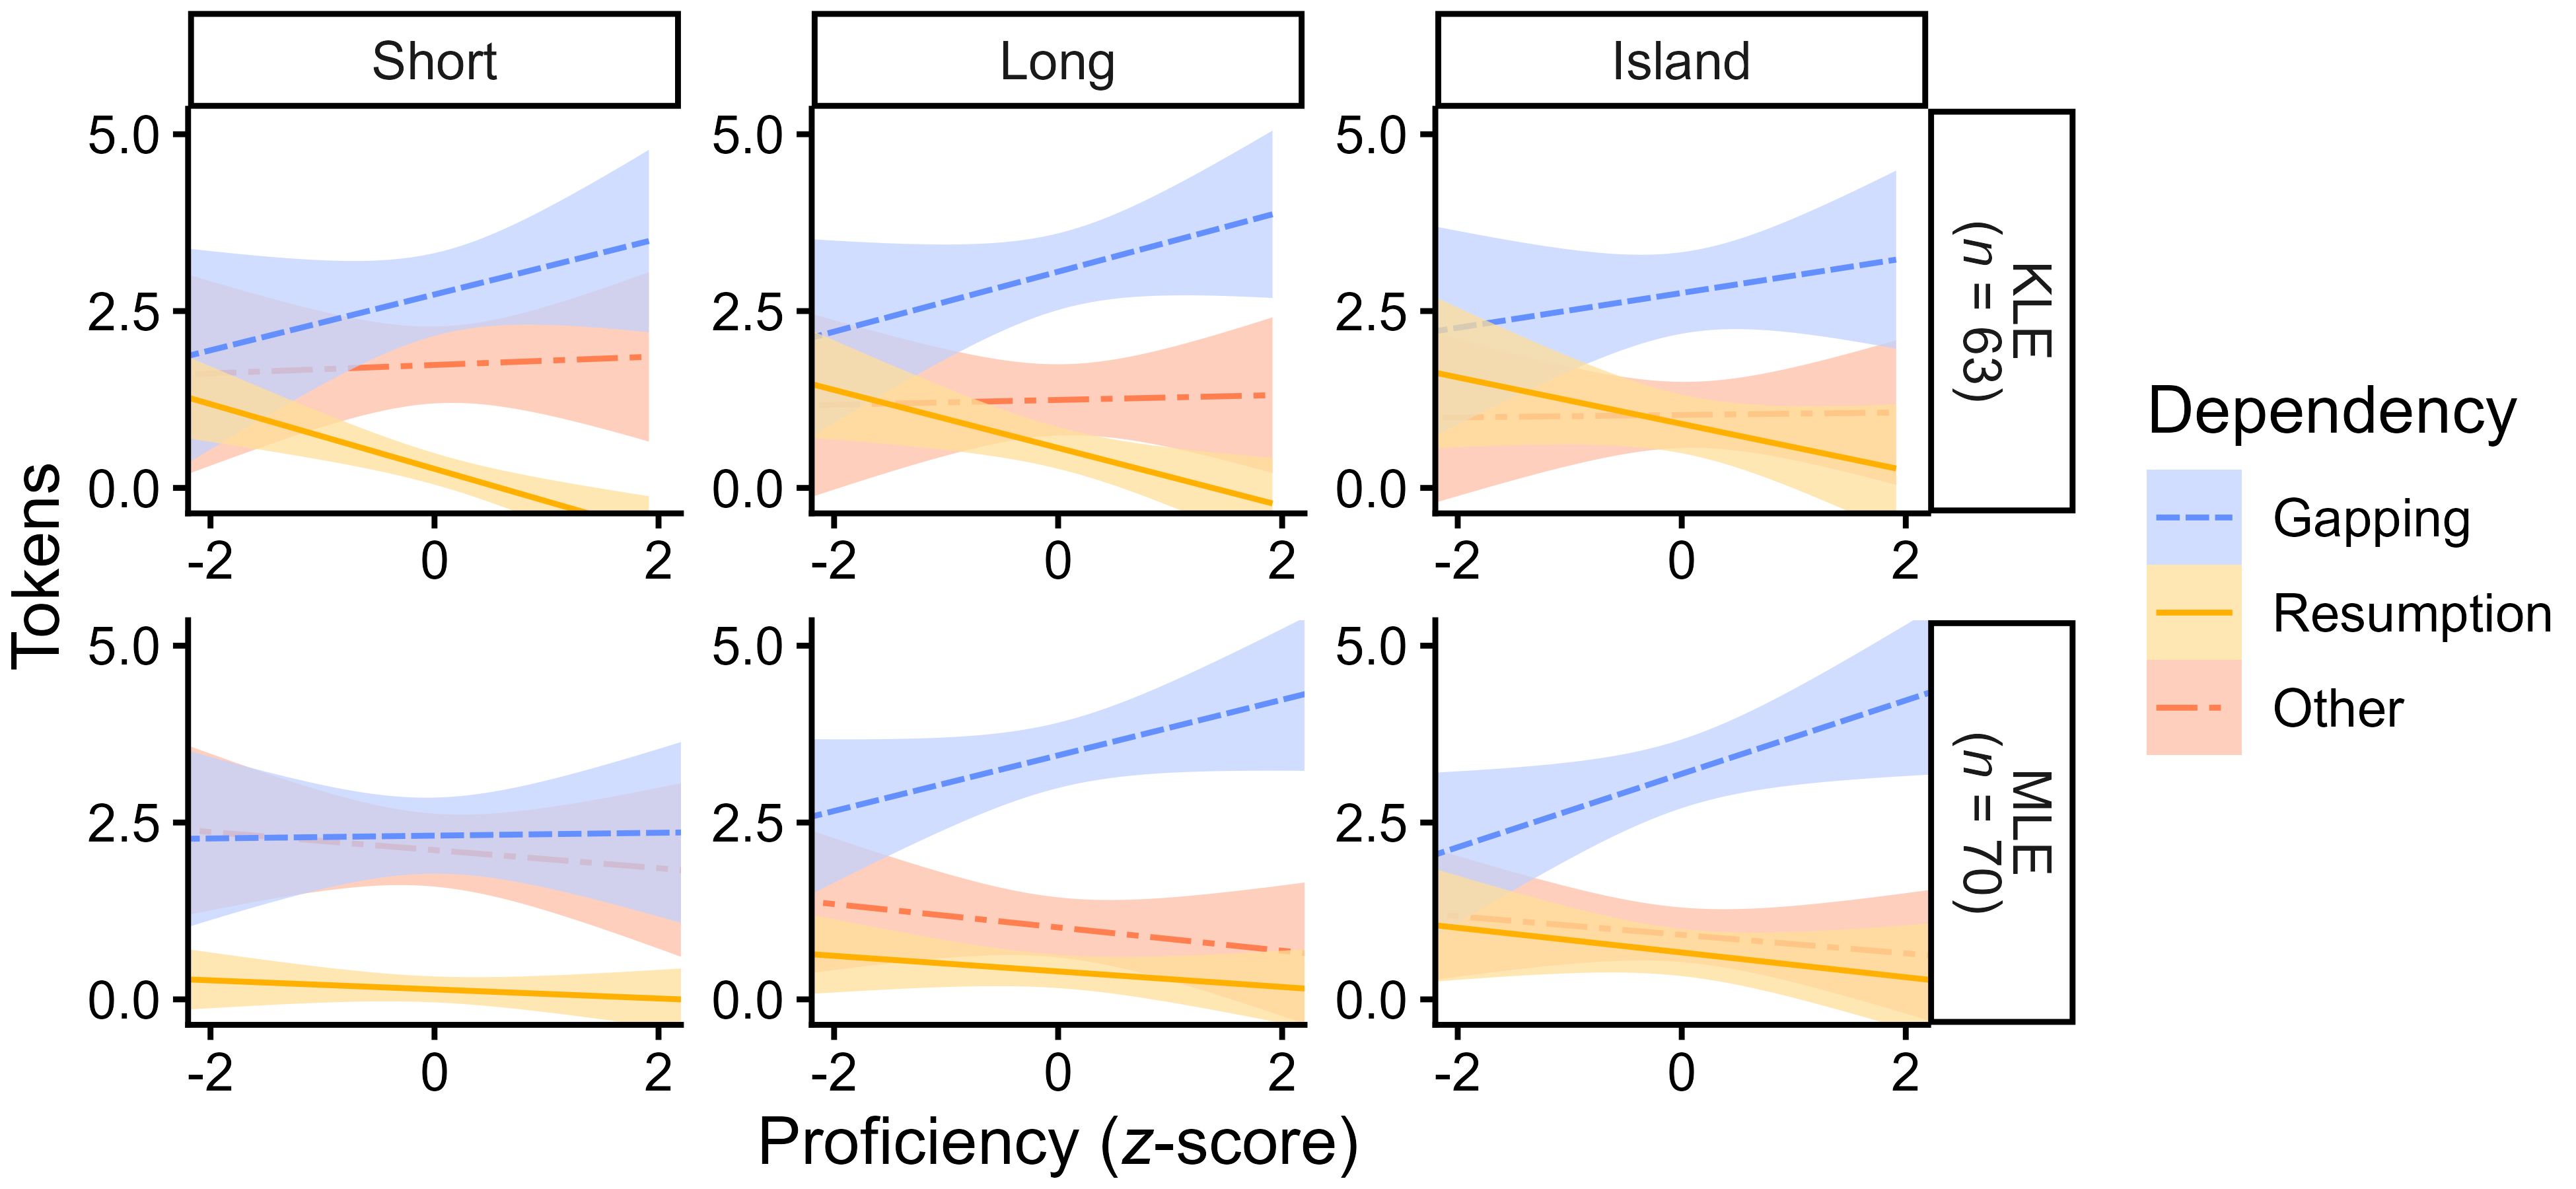
\includegraphics{../analysis/plots/orc_ept_token_proficiency.png}
% \textit{Note}. Shading indicates 95\% $CI$s.
% \vspace{-12pt}
% \end{figure}

% SRC Figure
% \begin{figure}
% \caption{Relationship between L2 proficiency and response rates in the SRC elicited production task} \label{fig:app-src-ept-token-proficiency}
% \raggedright\setstretch{1}
% 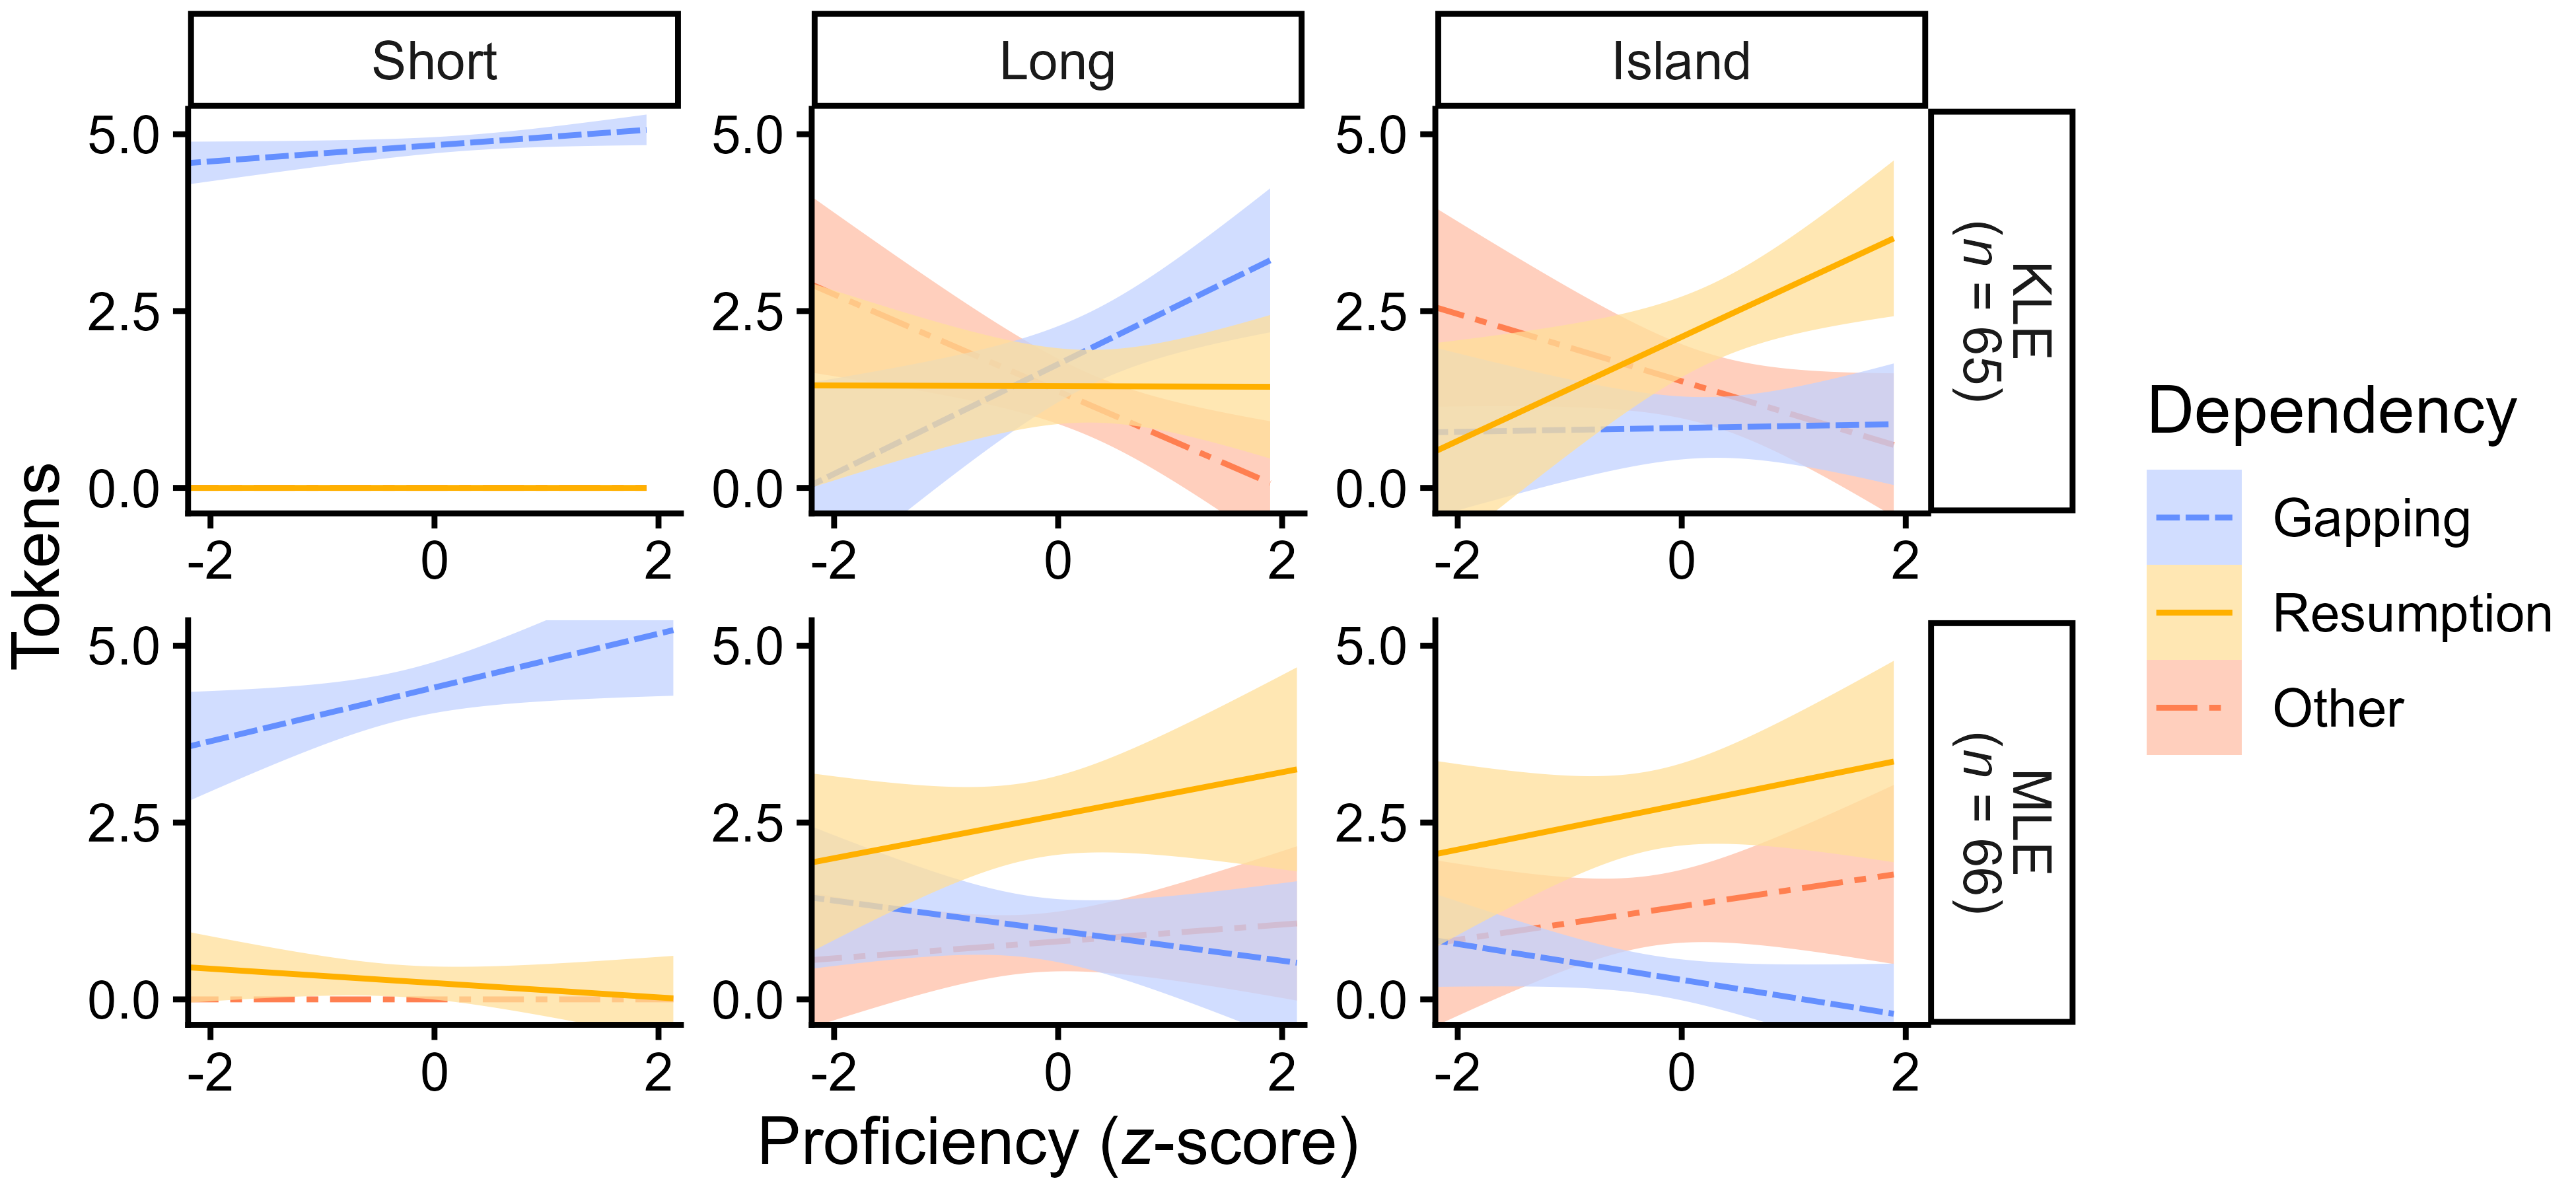
\includegraphics{../analysis/plots/src_ept_token_proficiency.png}
% \textit{Note}. Shading indicates 95\% $CI$s.
% \vspace{-12pt}
% \end{figure}

% ORC Model
\begin{table}
\caption{Summary of mixed-effects logistic regression model for L2 proficiency effects on resumption rates in the ORC elicited production task}\label{tab:app-orc-ept-resumption-proficiency-model}
\raggedright\setstretch{1}
\begin{tabularx}{\textwidth}{lYYYY}\toprule
Parameter & Estimate $\hat{\beta}$ & \textit{SE} & $z$ & $p$ \\\midrule
\csvreader[late after line=\\,late after last line=\\\bottomrule]
{../analysis/tables/orc_ept_resumption_proficiency_model.csv}{}{\csvcoli & \csvcolii & \csvcoliii & \csvcoliv & \csvcolv}
\end{tabularx}
\textit{Note}. Model formula: Resumption \~{} Environment * Group * Proficiency + (1 + Environment | Participant) + (1 + Environment + Group | Item); reference level: Short + ENS; estimate unit: logit; intercept: grand mean.
\vspace{-12pt}
\end{table}

% ORC Posthoc
\begin{table}
\caption{Post-hoc tests for L2 proficiency trend in the ORC elicited production task}\label{tab:app-orc-ept-proficiency-posthoc}
\raggedright\setstretch{1}
\begin{tabularx}{\textwidth}{llYYYY}\toprule
Group~~ & Contrast & Estimate $\hat{\beta}$ & \textit{SE} & $z$ & $p$ \\\midrule
\csvreader[late after line=\\,late after last line=\\\bottomrule]
{../analysis/tables/orc_ept_proficiency_posthoc.csv}{}{\csvcoli & \csvcolii & \csvcoliii & \csvcoliv & \csvcolv & \csvcolvi}
\end{tabularx}
\textit{Note}. Adjustment to $p$-values done via multiple $t$ method for 6 tests.
\vspace{-12pt}
\end{table}

% SRC Model
\begin{table}
\caption{Summary of mixed-effects logistic regression model for L2 proficiency effects on resumption rates in the SRC elicited production task}\label{tab:app-src-ept-resumption-proficiency-model}
\raggedright\setstretch{1}
\begin{tabularx}{\textwidth}{lYYYY}\toprule
Parameter & Estimate $\hat{\beta}$ & \textit{SE} & $z$ & $p$ \\\midrule
\csvreader[late after line=\\,late after last line=\\\bottomrule]
{../analysis/tables/src_ept_resumption_proficiency_model.csv}{}{\csvcoli & \csvcolii & \csvcoliii & \csvcoliv & \csvcolv}
\end{tabularx}
\textit{Note}. Model formula: Resumption \~{} Environment * Group * Proficiency + (1 + Environment | Participant) + (1 | Item); reference level: Short + ENS; estimate unit: logit; intercept: grand mean.
\vspace{-12pt}
\end{table}

% SRC Posthoc
\begin{table}
\caption{Post-hoc tests for L2 proficiency trend in the SRC elicited production task}\label{tab:app-src-ept-proficiency-posthoc}
\raggedright\setstretch{1}
\begin{tabularx}{\textwidth}{llYYYY}\toprule
Group~~ & Contrast & Estimate $\hat{\beta}$ & \textit{SE} & $z$ & $p$ \\\midrule
\csvreader[late after line=\\,late after last line=\\\bottomrule]
{../analysis/tables/src_ept_proficiency_posthoc.csv}{}{\csvcoli & \csvcolii & \csvcoliii & \csvcoliv & \csvcolv & \csvcolvi}
\end{tabularx}
\textit{Note}. Adjustment to $p$-values done via multiple $t$ method for 6 tests.
\vspace{-12pt}
\end{table}

%========================================================%
\section{Spread of response types across participants}\label{app-ept-spread}
%========================================================%

% ORC Proportions
% \DTLloaddb{dt-ept-prop}{../analysis/tables/ept_prop.csv}
% \ExplSyntaxOn
% \tl_clear:N \tblrbody
% \tl_build_begin:N \tblrbody
% \DTLforeach[\equal{\study}{ORC}]{dt-ept-prop}{\study=study,\coli=Group,\colii=Environment,\coliii=Dependency,\coliv=Percent}{\tl_build_put_right:Ne \tblrbody {\exp_not:V \coli & \exp_not:V \colii & \exp_not:V \coliii & \exp_not:V \coliv\\}}
% \tl_build_end:N \tblrbody
% \ExplSyntaxOff
% \begin{longtblr}[caption={Spread of response types across participants in the ORC elicited production task}, label={tblr:app-orc-ept-prop}, expand=\tblrbody]{colspec={XXXX[r]}}\toprule
% Group & Environment & Dependency & Participants (\%)\\\midrule
% \tblrbody\bottomrule
% \end{longtblr}
% \vspace{-12pt}

% SRC Proportions
% \ExplSyntaxOn
% \tl_clear:N \tblrbody
% \tl_build_begin:N \tblrbody
% \DTLforeach[\equal{\study}{SRC}]{dt-ept-prop}{\study=study,\coli=Group,\colii=Environment,\coliii=Dependency,\coliv=Percent}{\tl_build_put_right:Ne \tblrbody {\exp_not:V \coli & \exp_not:V \colii & \exp_not:V \coliii & \exp_not:V \coliv\\}}
% \tl_build_end:N \tblrbody
% \ExplSyntaxOff
% \begin{longtblr}[caption={Spread of response types across participants in the SRC elicited production task}, label={tblr:app-src-ept-prop}, expand=\tblrbody]{colspec={XXXX[r]}}\toprule
% Group & Environment & Dependency & Participants (\%)\\\midrule
% \tblrbody\bottomrule
% \end{longtblr}
% \vspace{-12pt}

% ORC Figure
\begin{figure}
\caption{Spread of response types across participants in the ORC elicited production task} \label{fig:app-orc-ept-prop}
\raggedright\setstretch{1}
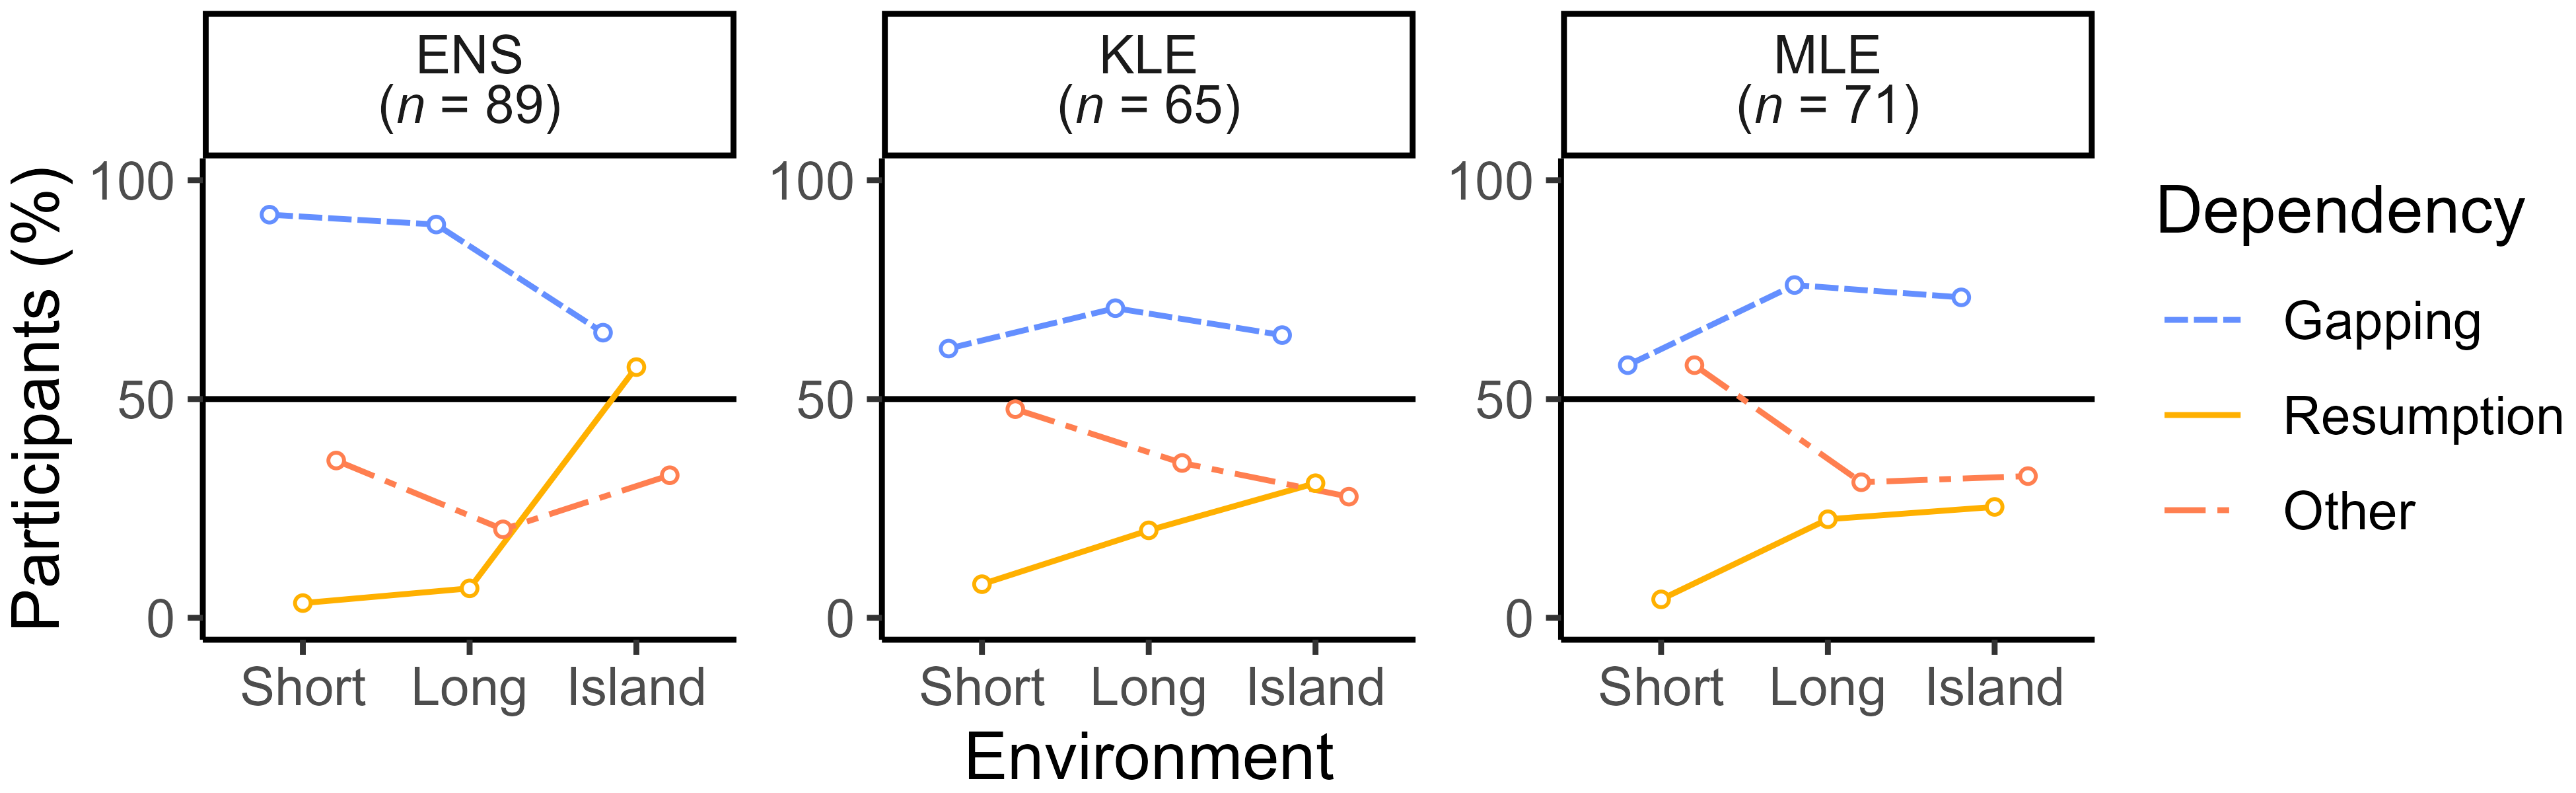
\includegraphics{../analysis/plots/orc_ept_prop.png}
\vspace{-12pt}
\end{figure}

% SRC Figure
\begin{figure}
\caption{Spread of response types across participants in the SRC elicited production task} \label{fig:app-src-ept-prop}
\raggedright\setstretch{1}
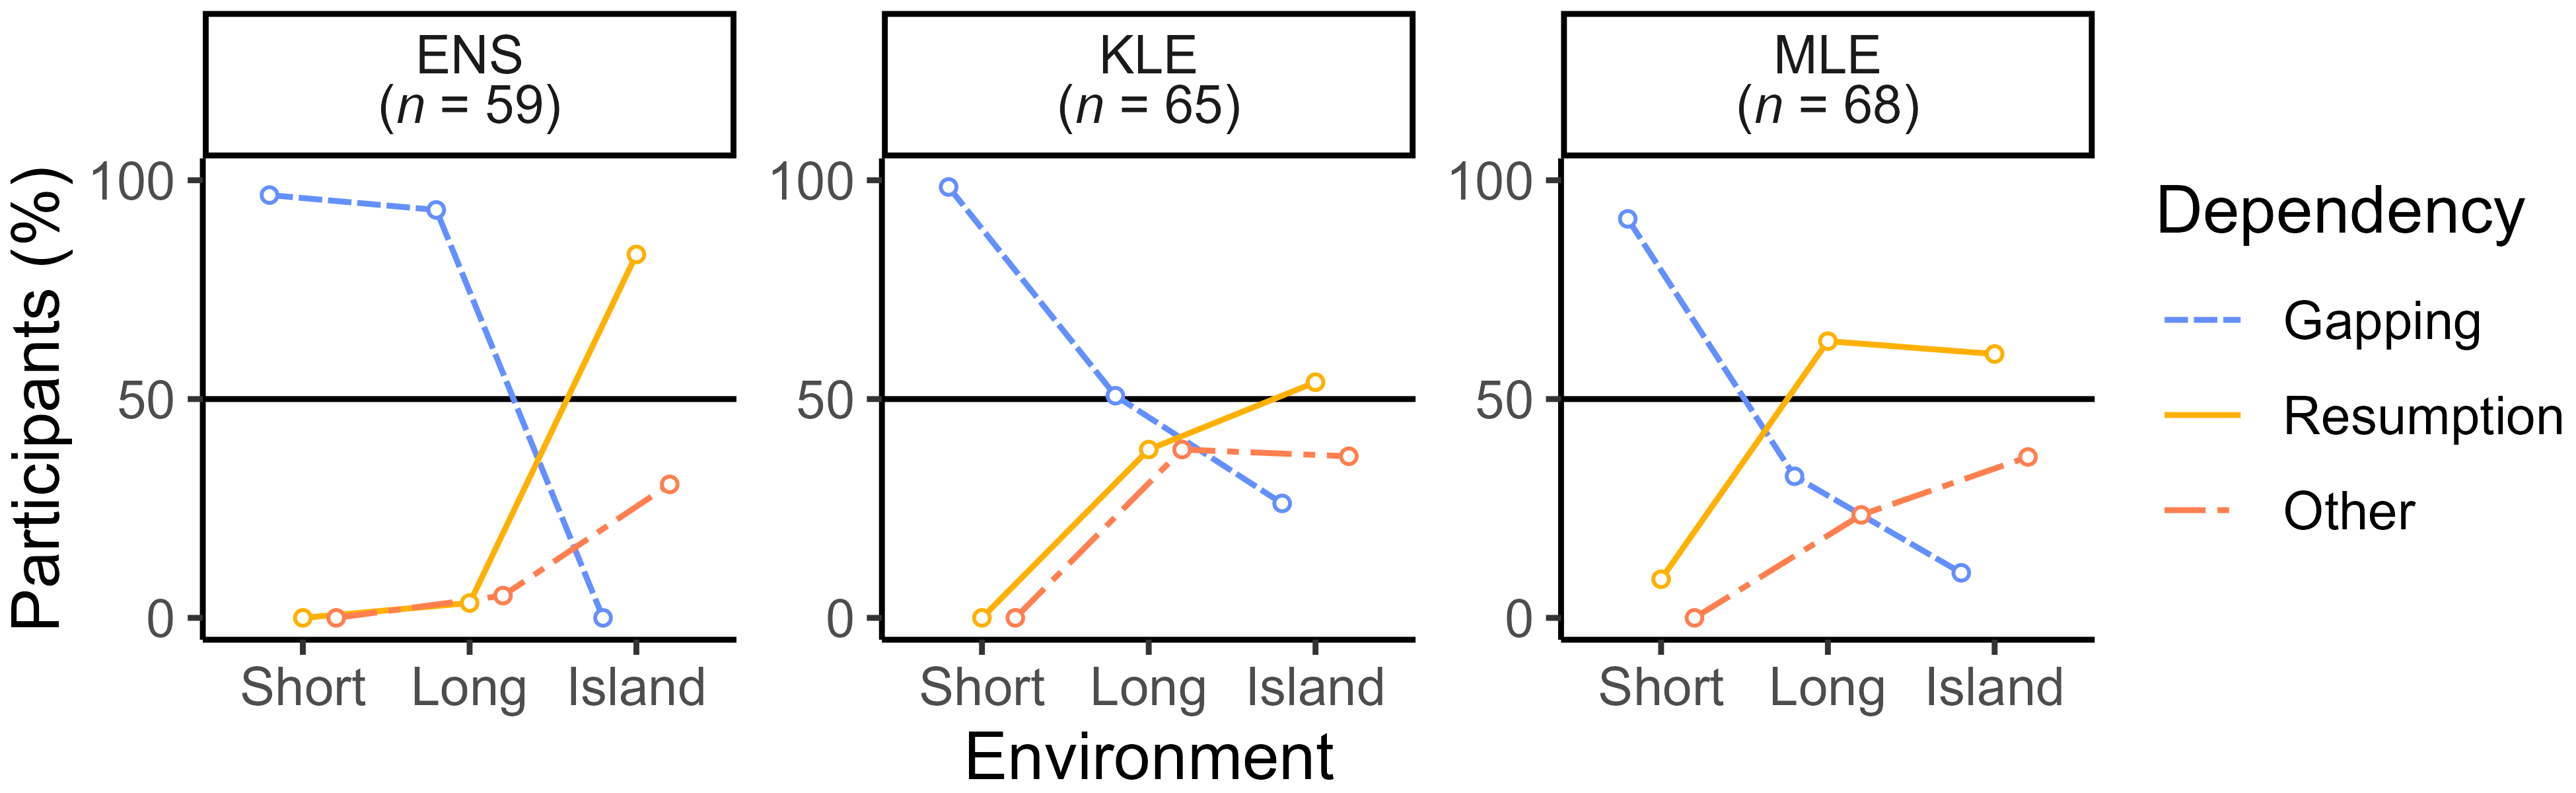
\includegraphics{../analysis/plots/src_ept_prop.png}
\end{figure}

%========================================================%
\section{Response tokens for fillers}\label{app-ept-token-filler}
%========================================================%

% ORC Means
% \DTLloaddb{dt-ept-token-filler}{../analysis/tables/ept_token_filler.csv}
% \ExplSyntaxOn
% \tl_clear:N \tblrbody
% \tl_build_begin:N \tblrbody
% \DTLforeach[\equal{\study}{ORC}]{dt-ept-token-filler}{\study=study,\coli=Group,\colii=Type,\coliii=Dependency,\coliv=Tokens,\colv=$CI$,\colvi=Percent}{\tl_build_put_right:Ne \tblrbody {\exp_not:V \coli & \exp_not:V \colii & \exp_not:V \coliii & \exp_not:V \coliv & \exp_not:V \colv & \exp_not:V \colvi\\}}
% \tl_build_end:N \tblrbody
% \ExplSyntaxOff
% \begin{longtblr}[caption={Mean tokens by participant for fillers in the ORC elicited production task}, label={tblr:app-orc-ept-token-filler}, expand=\tblrbody]{colspec={XXXX[r]X[r]X[r]}}\toprule
% Group & Type & Dependency & Mean & 95\% \textit{CI} & \%\\\midrule
% \tblrbody\bottomrule
% \end{longtblr}
% \vspace{-12pt}

% SRC Means
% \ExplSyntaxOn
% \tl_clear:N \tblrbody
% \tl_build_begin:N \tblrbody
% \DTLforeach[\equal{\study}{SRC}]{dt-ept-token-filler}{\study=study,\coli=Group,\colii=Type,\coliii=Dependency,\coliv=Tokens,\colv=$CI$,\colvi=Percent}{\tl_build_put_right:Ne \tblrbody {\exp_not:V \coli & \exp_not:V \colii & \exp_not:V \coliii & \exp_not:V \coliv & \exp_not:V \colv & \exp_not:V \colvi\\}}
% \tl_build_end:N \tblrbody
% \ExplSyntaxOff
% \begin{longtblr}[caption={Mean tokens by participant for fillers in the SRC elicited production task}, label={tblr:app-src-ept-token-filler}, expand=\tblrbody]{colspec={XXXX[r]X[r]X[r]}}\toprule
% Group & Type & Dependency & Mean & 95\% \textit{CI} & \%\\\midrule
% \tblrbody\bottomrule
% \end{longtblr}
% \vspace{-12pt}

% ORC Figure
\begin{figure}
\caption{Mean tokens by participant for fillers in the ORC elicited production task} \label{fig:app-orc-ept-token-filler}
\raggedright\setstretch{1}
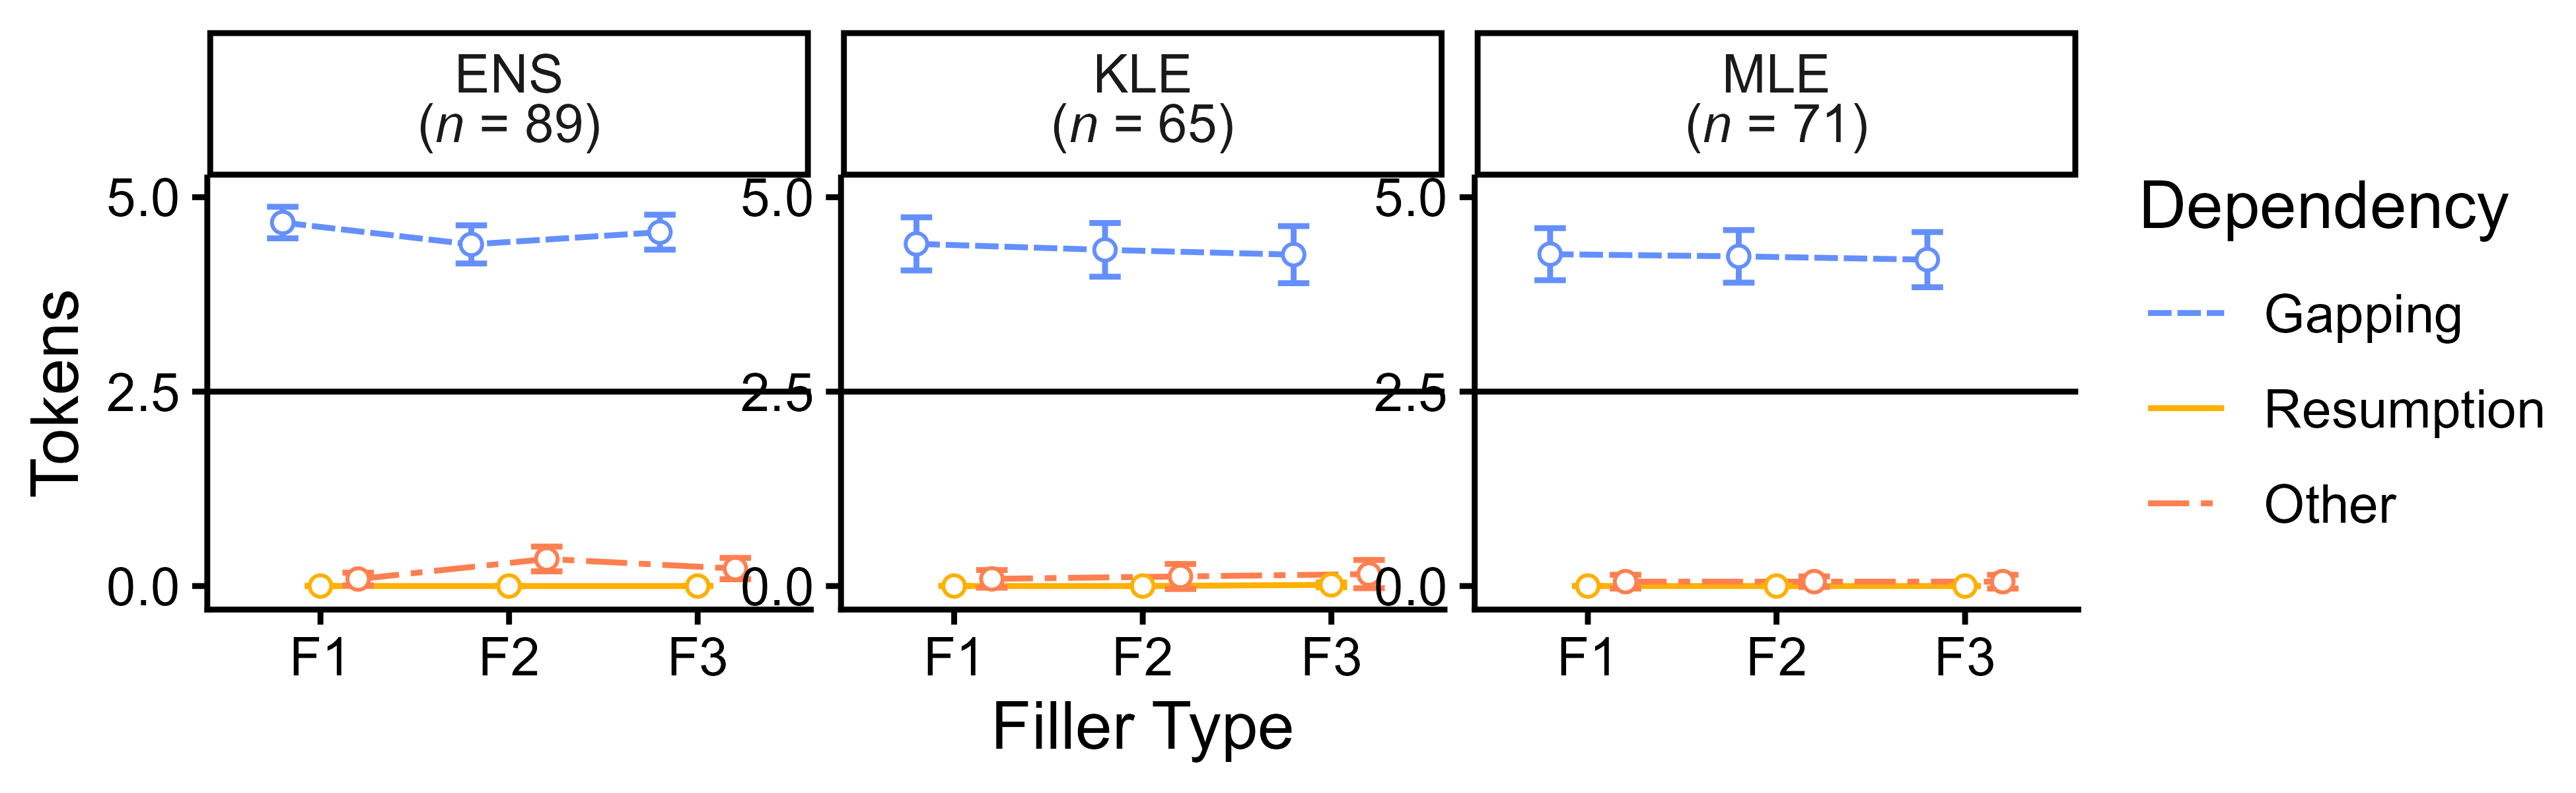
\includegraphics{../analysis/plots/orc_ept_token_filler.png}
\textit{Note}. Error bars are 95\% $CI$s; center line corresponds to a 50\% response rate.
\vspace{-12pt}
\end{figure}

% SRC Figure
\begin{figure}
\caption{Mean tokens by participant for fillers in the SRC elicited production task} \label{fig:app-src-ept-token-filler}
\raggedright\setstretch{1}
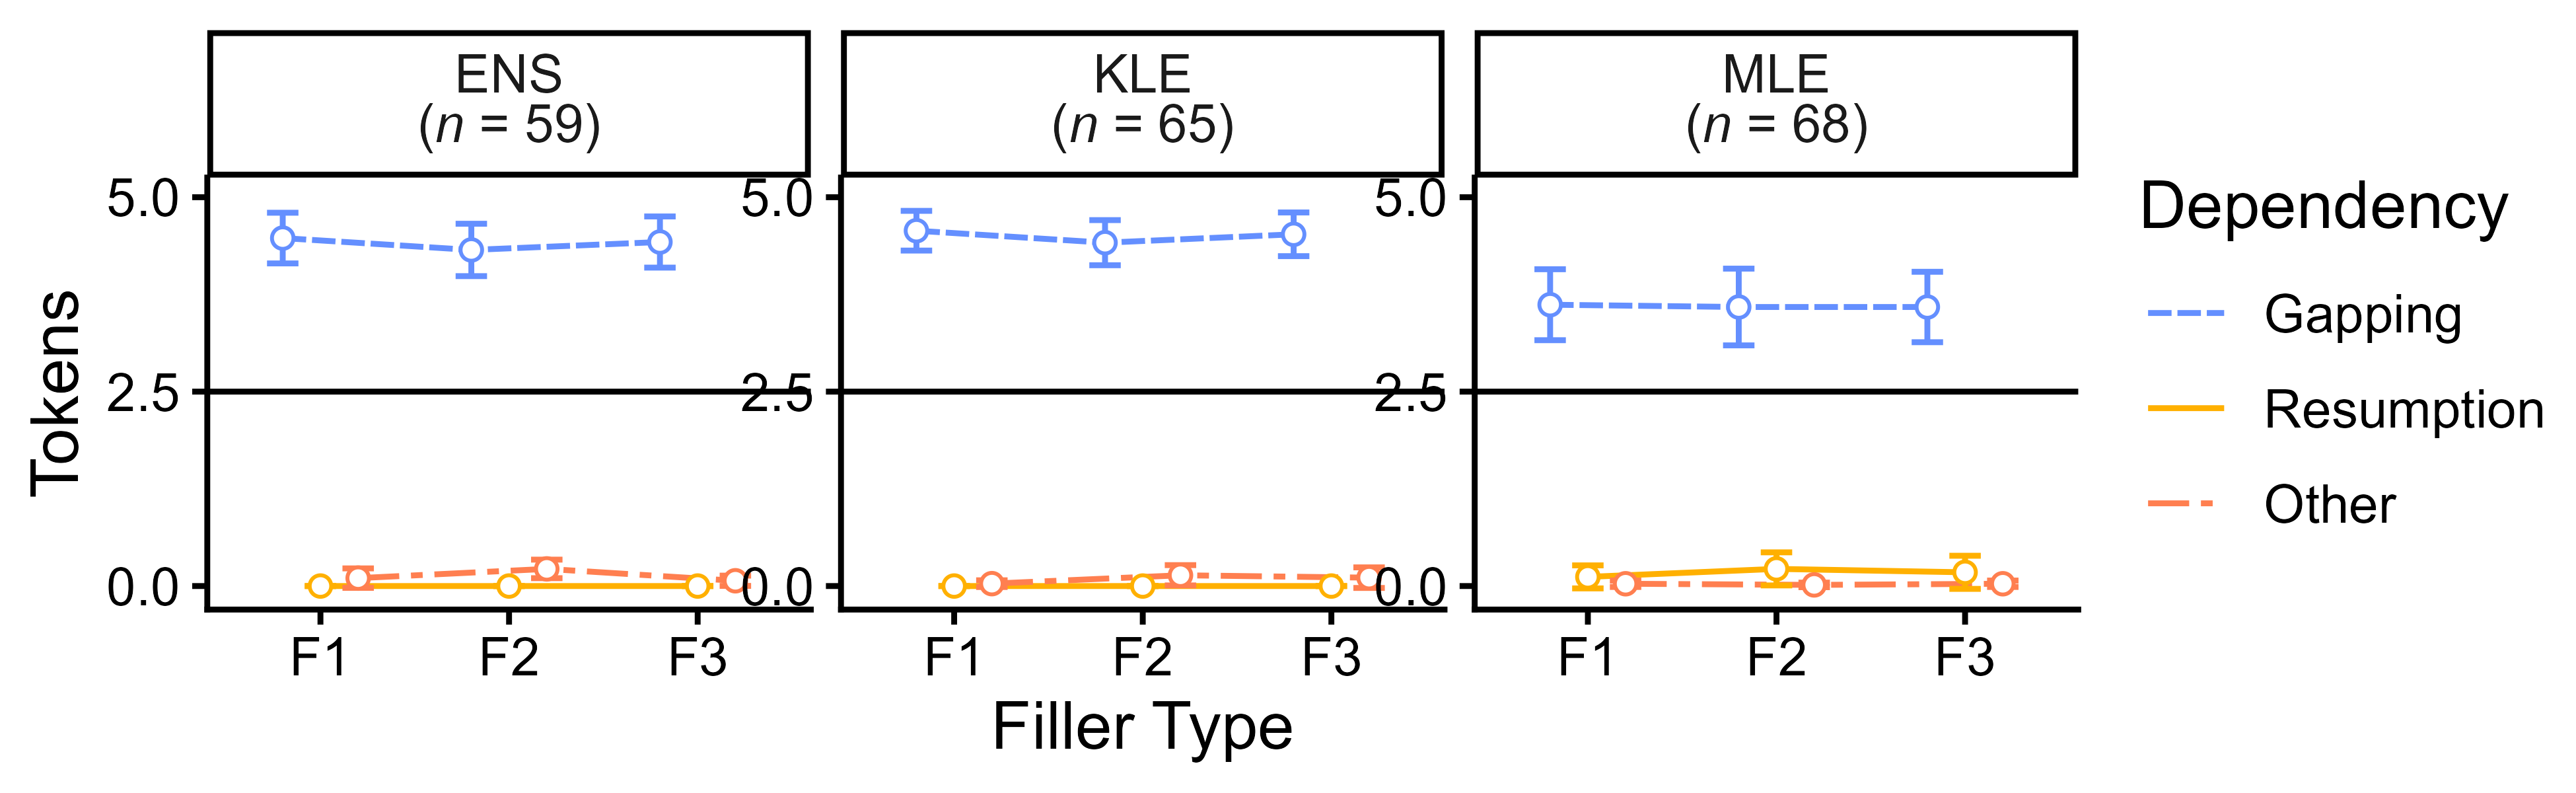
\includegraphics{../analysis/plots/src_ept_token_filler.png}
\textit{Note}. Error bars are 95\% $CI$s; center line corresponds to a 50\% response rate.
\vspace{-12pt}
\end{figure}